\documentclass{article}
\usepackage{graphicx}
\graphicspath{ {./images/} }

\title{Ch. 6.2 HW}
\author{Principles of Microeconomics}
\date{\today}

\begin{document}

\maketitle

\subsection*{Quick Quiz}

\begin{enumerate}

\item (a) -- The incidence of a tax doesn't depend on who pays the tax.

\item (d) --
	\begin{center}
	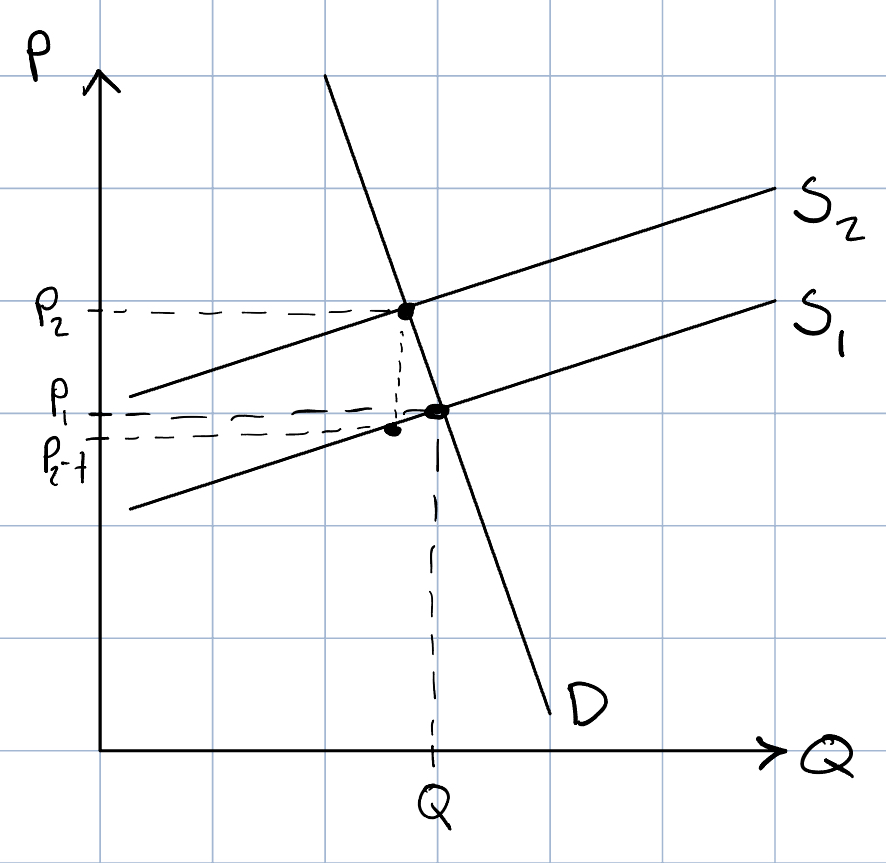
\includegraphics[width = 0.5\textwidth]{qq6}
	\end{center}

\item (c) --
	\begin{center}
	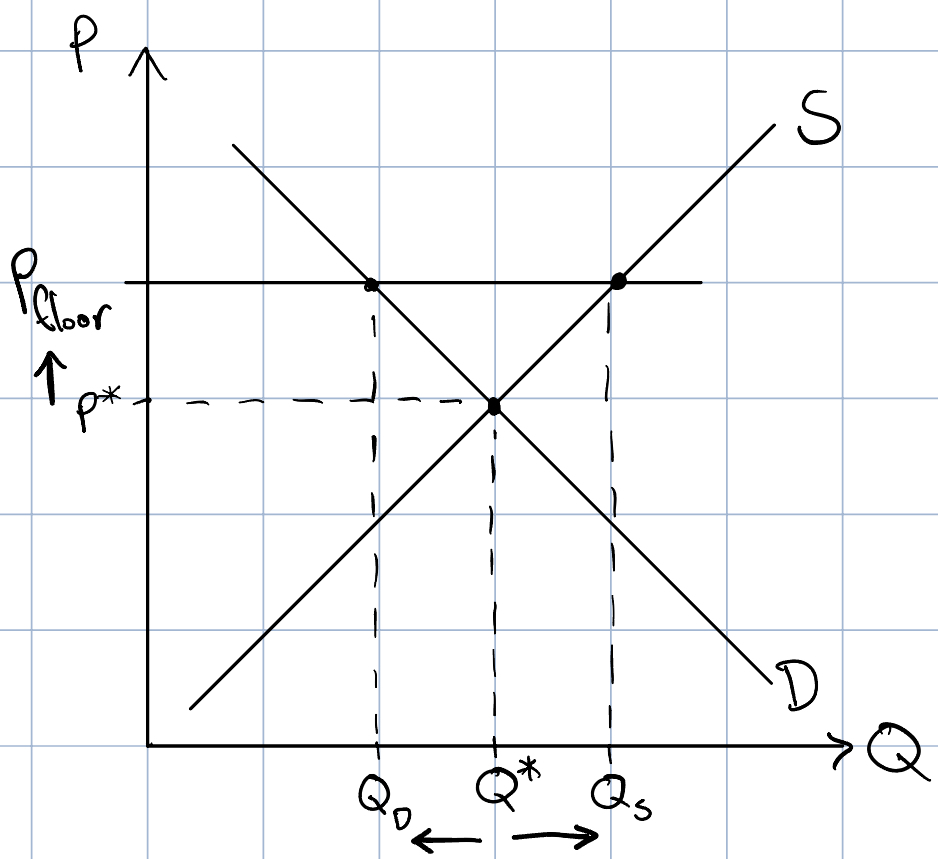
\includegraphics[width = 0.5\textwidth]{qq7}
	\end{center}

\item (b) --
	\begin{center}
	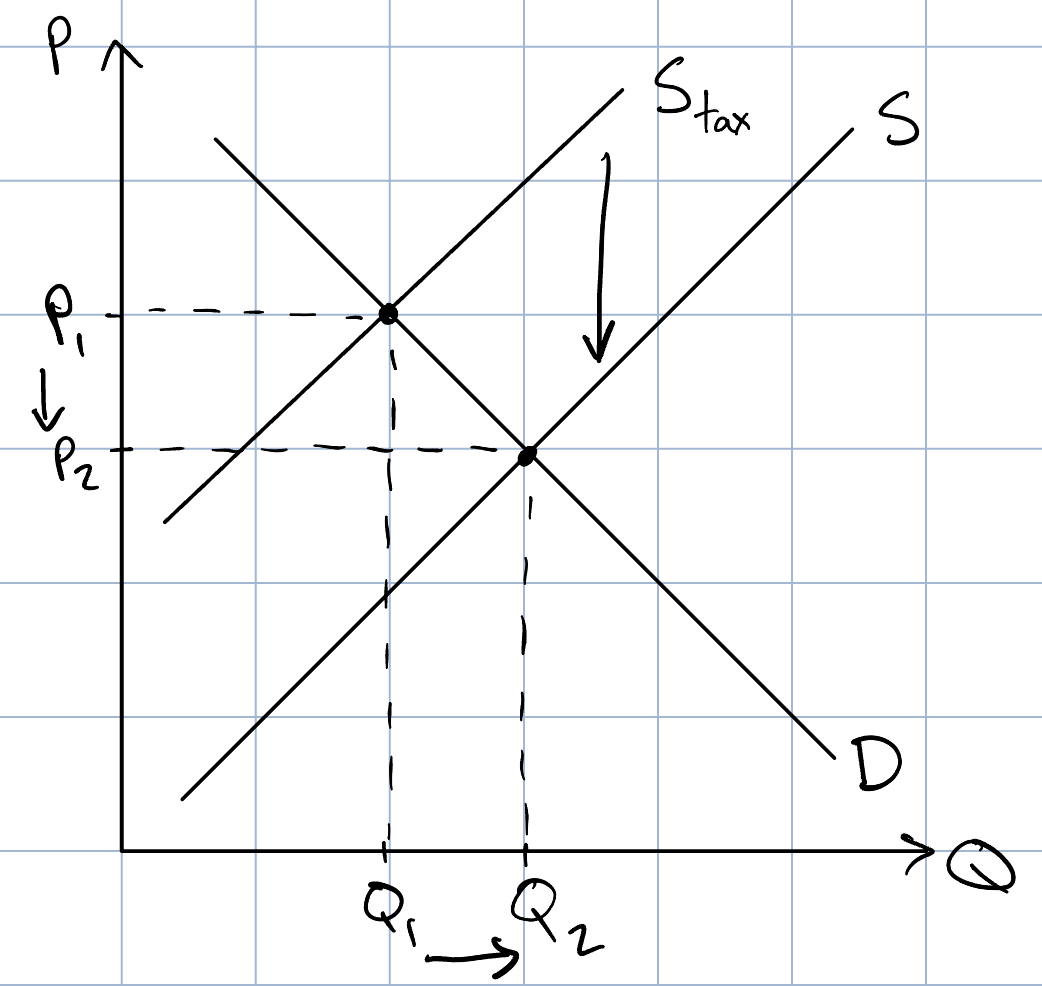
\includegraphics[width = 0.5\textwidth]{qq8}
	\end{center}

\end{enumerate}

\subsection*{Problems and Applications}

\begin{enumerate}
\setcounter{enumi}{3}

\item 

	\begin{enumerate}
	
	\item At the market equilibrium, there is no difference between the price paid by consumers and the price received by sellers. 
		\begin{center}
		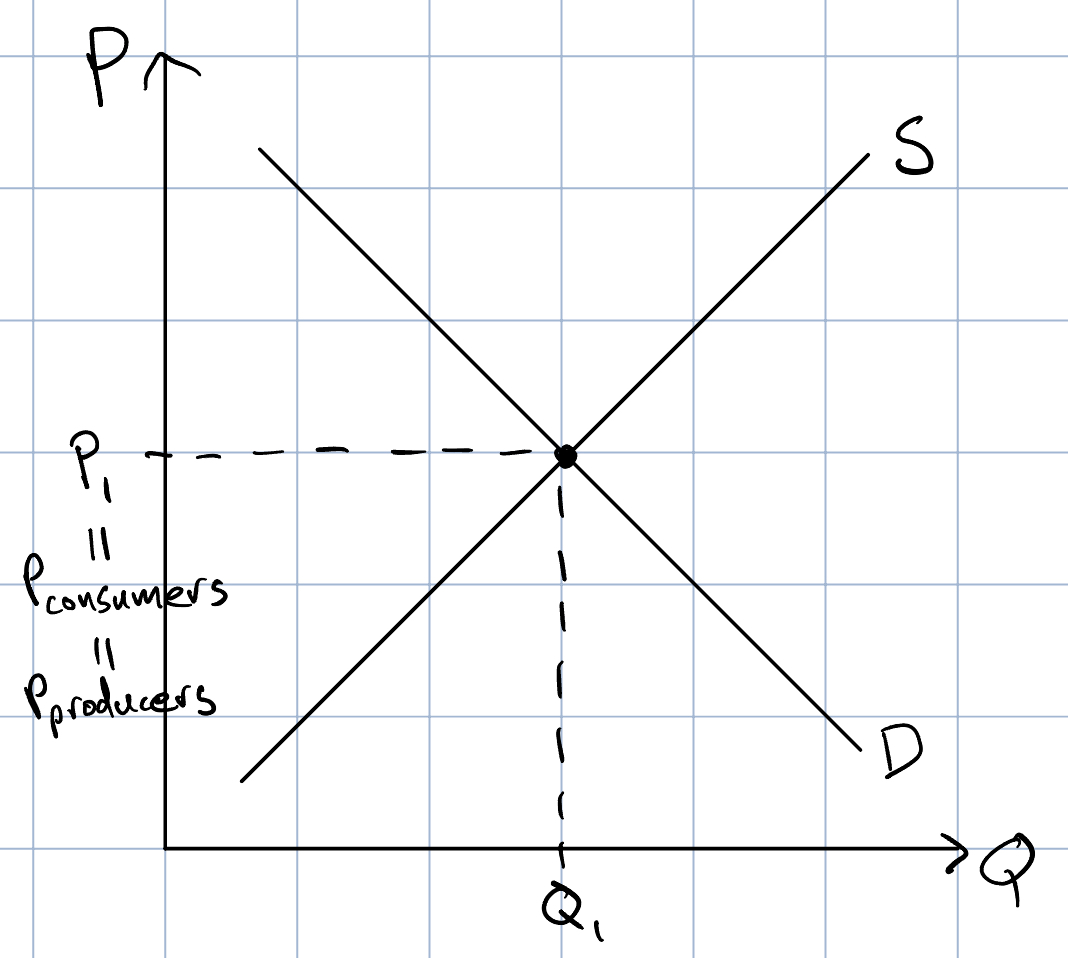
\includegraphics[width = 0.5\textwidth]{paa4a}
		\end{center}
		
	\newpage
	
	\item The difference between the price paid by consumers and the price received by sellers is the amount of the tax, \$2. 
		\begin{center}
		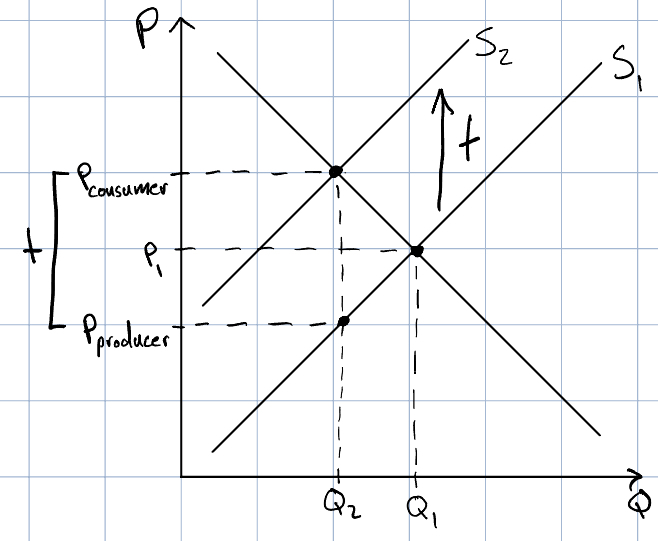
\includegraphics[width = 0.5\textwidth]{paa4b}
		\end{center}
	
	\end{enumerate}
	
\item It would likely raise revenue. Labor demand and supply are likely inelastic, so a higher tax won't decrease the quantity of labor sold very much. If the tax rate rises and the quantity sold doesn't decrease much, tax revenue should increase.
	\begin{center}
	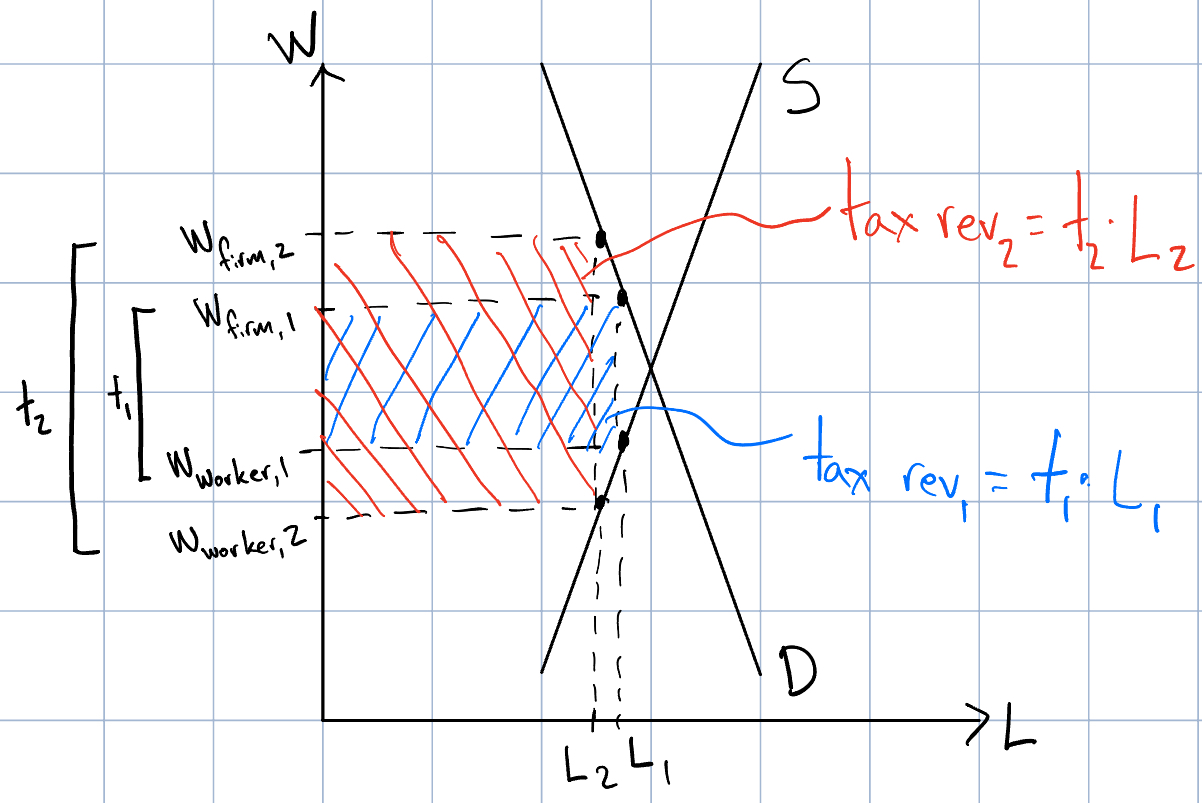
\includegraphics[width = 0.75\textwidth]{paa5_1}
	\end{center}
	
It wouldn't make workers better off. Who pays a tax doesn't determine the incidence of a tax. The elasticity of supply and demand determine the incidence of a tax. Since the policy does nothing to affect those two elasticities, it won't shift the incidence towards firms and away from workers. In fact, the tax will decrease the quantity of labor sold and decrease the wage workers receive, so it will make workers worse off.

\newpage

\item It will rise by less than \$500. Since neither the supply nor the demand for luxury cars is perfectly elastic or inelastic, the incidence of the tax will be split between consumers and producers.
	\begin{center}
	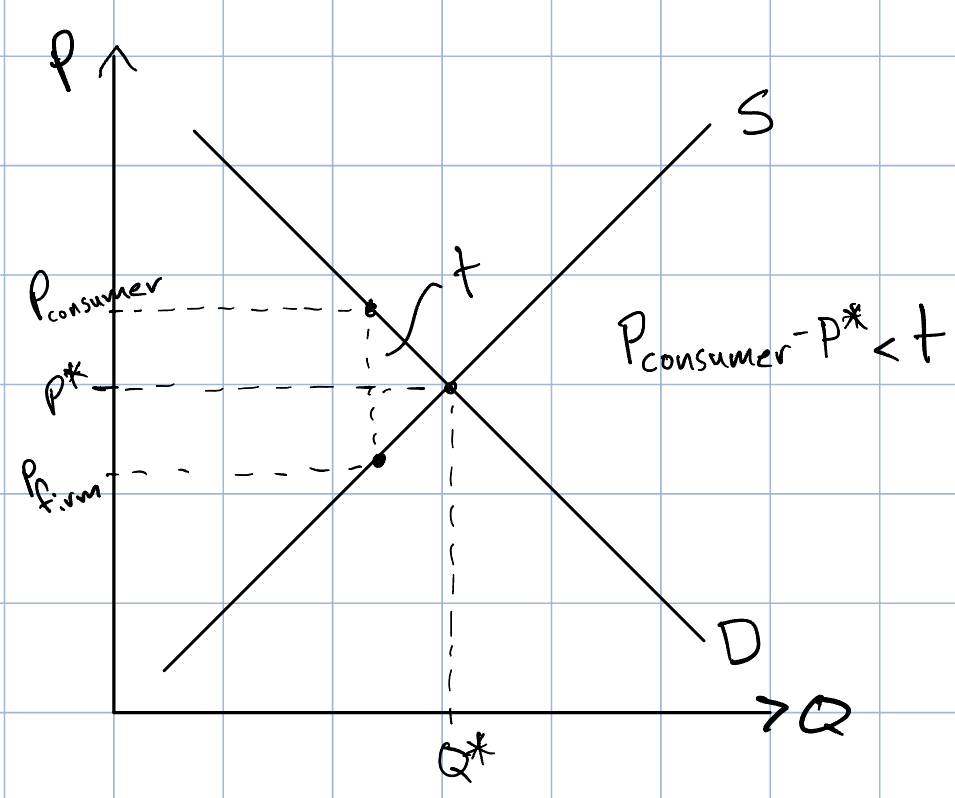
\includegraphics[width = 0.5\textwidth]{paa6}
	\end{center}
	
\item

	\begin{enumerate}
	
	\item
	
	\end{enumerate}

\end{enumerate}

\end{document}